%% Software Manual and Technical Document Template	
%% 									
%% This provides an example of a software manual created in Overleaf.

\documentclass{ol-softwaremanual}

% Packages used in this example
\usepackage{graphicx}  % for including images
\usepackage{microtype} % for typographical enhancements
% \usepackage{minted}    % for code listings
\usepackage{amsmath}   % for equations and mathematics
% \setminted{style=friendly,fontsize=\small}
% \renewcommand{\listoflistingscaption}{List of Code Listings}
\usepackage{hyperref}  % for hyperlinks
\usepackage[a4paper,top=4.2cm,bottom=4.2cm,left=3.5cm,right=3.5cm]{geometry}
\usepackage{authblk}
\usepackage{pdfsync}
\usepackage{boldline}
\usepackage{longtable}
\usepackage[version=3]{acro}
\usepackage{gensymb}
% \usepackage[printonlyused,withpage]{acronym}
\usepackage[numbers,sort&compress]{natbib}
\usepackage{anysize}
% \marginsize{2cm}{2cm}{1.cm}               {1.cm}
\usepackage{graphicx}
\usepackage{epsfig}
\usepackage{verbatim} 
\usepackage{bm}
\usepackage{etoolbox}
%\usepackage{amssymb}
%\usepackage{amsfonts,amsmath}
\usepackage{multirow}
% \usepackage[T1]{fontenc}
\usepackage{yfonts}
\usepackage{xr-hyper} 
% \externaldocument{manuscript}
\usepackage{xcite} 
% \externalcitedocument{manuscript}
\usepackage{mathrsfs}
% \usepackage{fancyhdr}
% \usepackage{relsize}
%  \usepackage{newpxtext,newpxmath}
%  \usepackage{booktabs,siunitx}
\usepackage{array,booktabs,ragged2e}
\usepackage{enumitem}   
\usepackage{empheq}
\usepackage[font=small,labelfont=bf]{caption}
\usepackage[title,toc,titletoc,page]{appendix}
\usepackage[capitalise]{cleveref}
\usepackage[most]{tcolorbox}
\usepackage{tocloft}
\usepackage{eurosym}
% \usepackage[colorlinks]{hyperref}

 % for setting page size and margins

% Custom macros used in this example document
\newcommand{\doclink}[2]{\href{#1}{#2}\footnote{\url{#1}}}
\newcommand{\cs}[1]{\texttt{\textbackslash #1}}

\acsetup{
  make-links ,
  pages / display = first ,
  pages / fill    = {, }
}

\hypersetup{colorlinks=true,
	linkcolor=blue,
	anchorcolor=black,
	citecolor=red,
	urlcolor=blue
}

\DeclareAcronym{UTC}{short = UTC, long = Universal Time Coordinated}
\DeclareAcronym{TAI}{short = TAI, long = International Atomic Time}
\DeclareAcronym{nm}{
    short = nm, 
    short-plural-form = {nm},
    long = nautical mile
    }
\DeclareAcronym{km}{
        short = km, 
        short-plural-form = {km},
        long = kilometer
}
\DeclareAcronym{hr}{
        short = h, 
        short-plural-form = {hrs},
        long = hour
}
\DeclareAcronym{min}{
        short = min, 
        short-plural-form = {mins},
        long = minute
}
\DeclareAcronym{sec}{
        short = s, 
        short-plural-form = {s},
        long = second
}
\DeclareAcronym{kt}{
    short = kt, 
    short-plural-form = {kts},
    long = knot
    }
\DeclareAcronym{ft}{
    short = ft, 
    short-plural-form = {ft},
    long = foot,
    long-plural-form = {feet}
    }
\DeclareAcronym{m}{
    short = m, 
    short-plural-form = {m},
    long = meter
    }

\DeclareAcronym{N}{
    short = N, 
    long = North
}
\DeclareAcronym{S}{
    short = N, 
    long = South
}
\DeclareAcronym{E}{
    short = E, 
    long = East
}
\DeclareAcronym{W}{
    short = W, 
    long = West
}
\providecommand{\thel}{Thelemacus\,\,}


% Frontmatter data; appears on title page
\title{Documentation}
\version{1.0}
\author{Michele Castellana}
\softwarelogo{\includegraphics[width=8cm]{logo}}

\begin{document}

\maketitle

\tableofcontents
% \listoflistings
\newpage

\section{Introduction}


\thel  is a navigational-astronomy application, which allows to compute one's position on the surface of the Earth, on both land and sea, based on sextant measurements. \thel is conceived to make the user's life easy, and it is designed for an intuitive and quick use. 

\subsection{Thelemacus is free software}

\thel is ``free software''; this means that everyone is free to use it. The software is not in the public domain \cite{castellana2024thelemacus}; it is copyrighted and there are conditions on its distribution. These conditions are designed to permit everything that a good cooperating citizen would want to do.

\subsection{Obtaining Thelemacus}

The source code for the library can be obtained from the GitHub repository \href{https://github.com/mcastel1/thelemacus}{mcastel1/thelemacus}. The executable can be downloaded from my \href{https://sites.google.com/site/michelecastellana/home}{website}, for OSx and Windows.  

Announcements of new releases, updates and other relevant events are made \href{https://sites.google.com/site/michelecastellana/home}{online}. 

\subsection{No warranty}

The \thel has no warranty, it is provided ``as is.'' It is your responsibility to validate the behavior of \thel and its accuracy using the source code provided, or to purchase support and warranties from commercial redistributors. Consult \thel's  License for further details.

\subsection{Reporting bugs}

A list of known bugs can be found in the \href{https://github.com/mcastel1/thelemacus/issues}{issues} section of the GitHub repository.
If you find a bug which is not listed in there, please report it to \href{mailto:michele.castellana@gmail.com}{me}. All bug reports should include:
\begin{itemize}
    \item The version number of \thel, 
    \item The hardware and operating system, 
    \item A short description of the bug behavior. 

\end{itemize}

Any errors or omissions in this manual can also be reported to the same address.


\subsection{Further information}


Additional information, including online copies of this manual, links to related projects, and mailing list archives are available from the \href{https://sites.google.com/site/michelecastellana/home}{website}  above.
Any questions about the use and installation of \thel can be asked by \href{mailto:michele.castellana@gmail.com}{email}. This mailing address can be used to ask questions not covered by this manual, and to contact the developers of the library.

If you would like to refer to \thel in a journal article, the recommended way is to cite this reference manual \cite{castellana2024thelemacus-documentation}. If you want to give a url, use  \href{https://sites.google.com/site/michelecastellana/home}{this one}. 


\pagebreak

\section{\thel for the impatient}

\begin{figure}
  \centering
  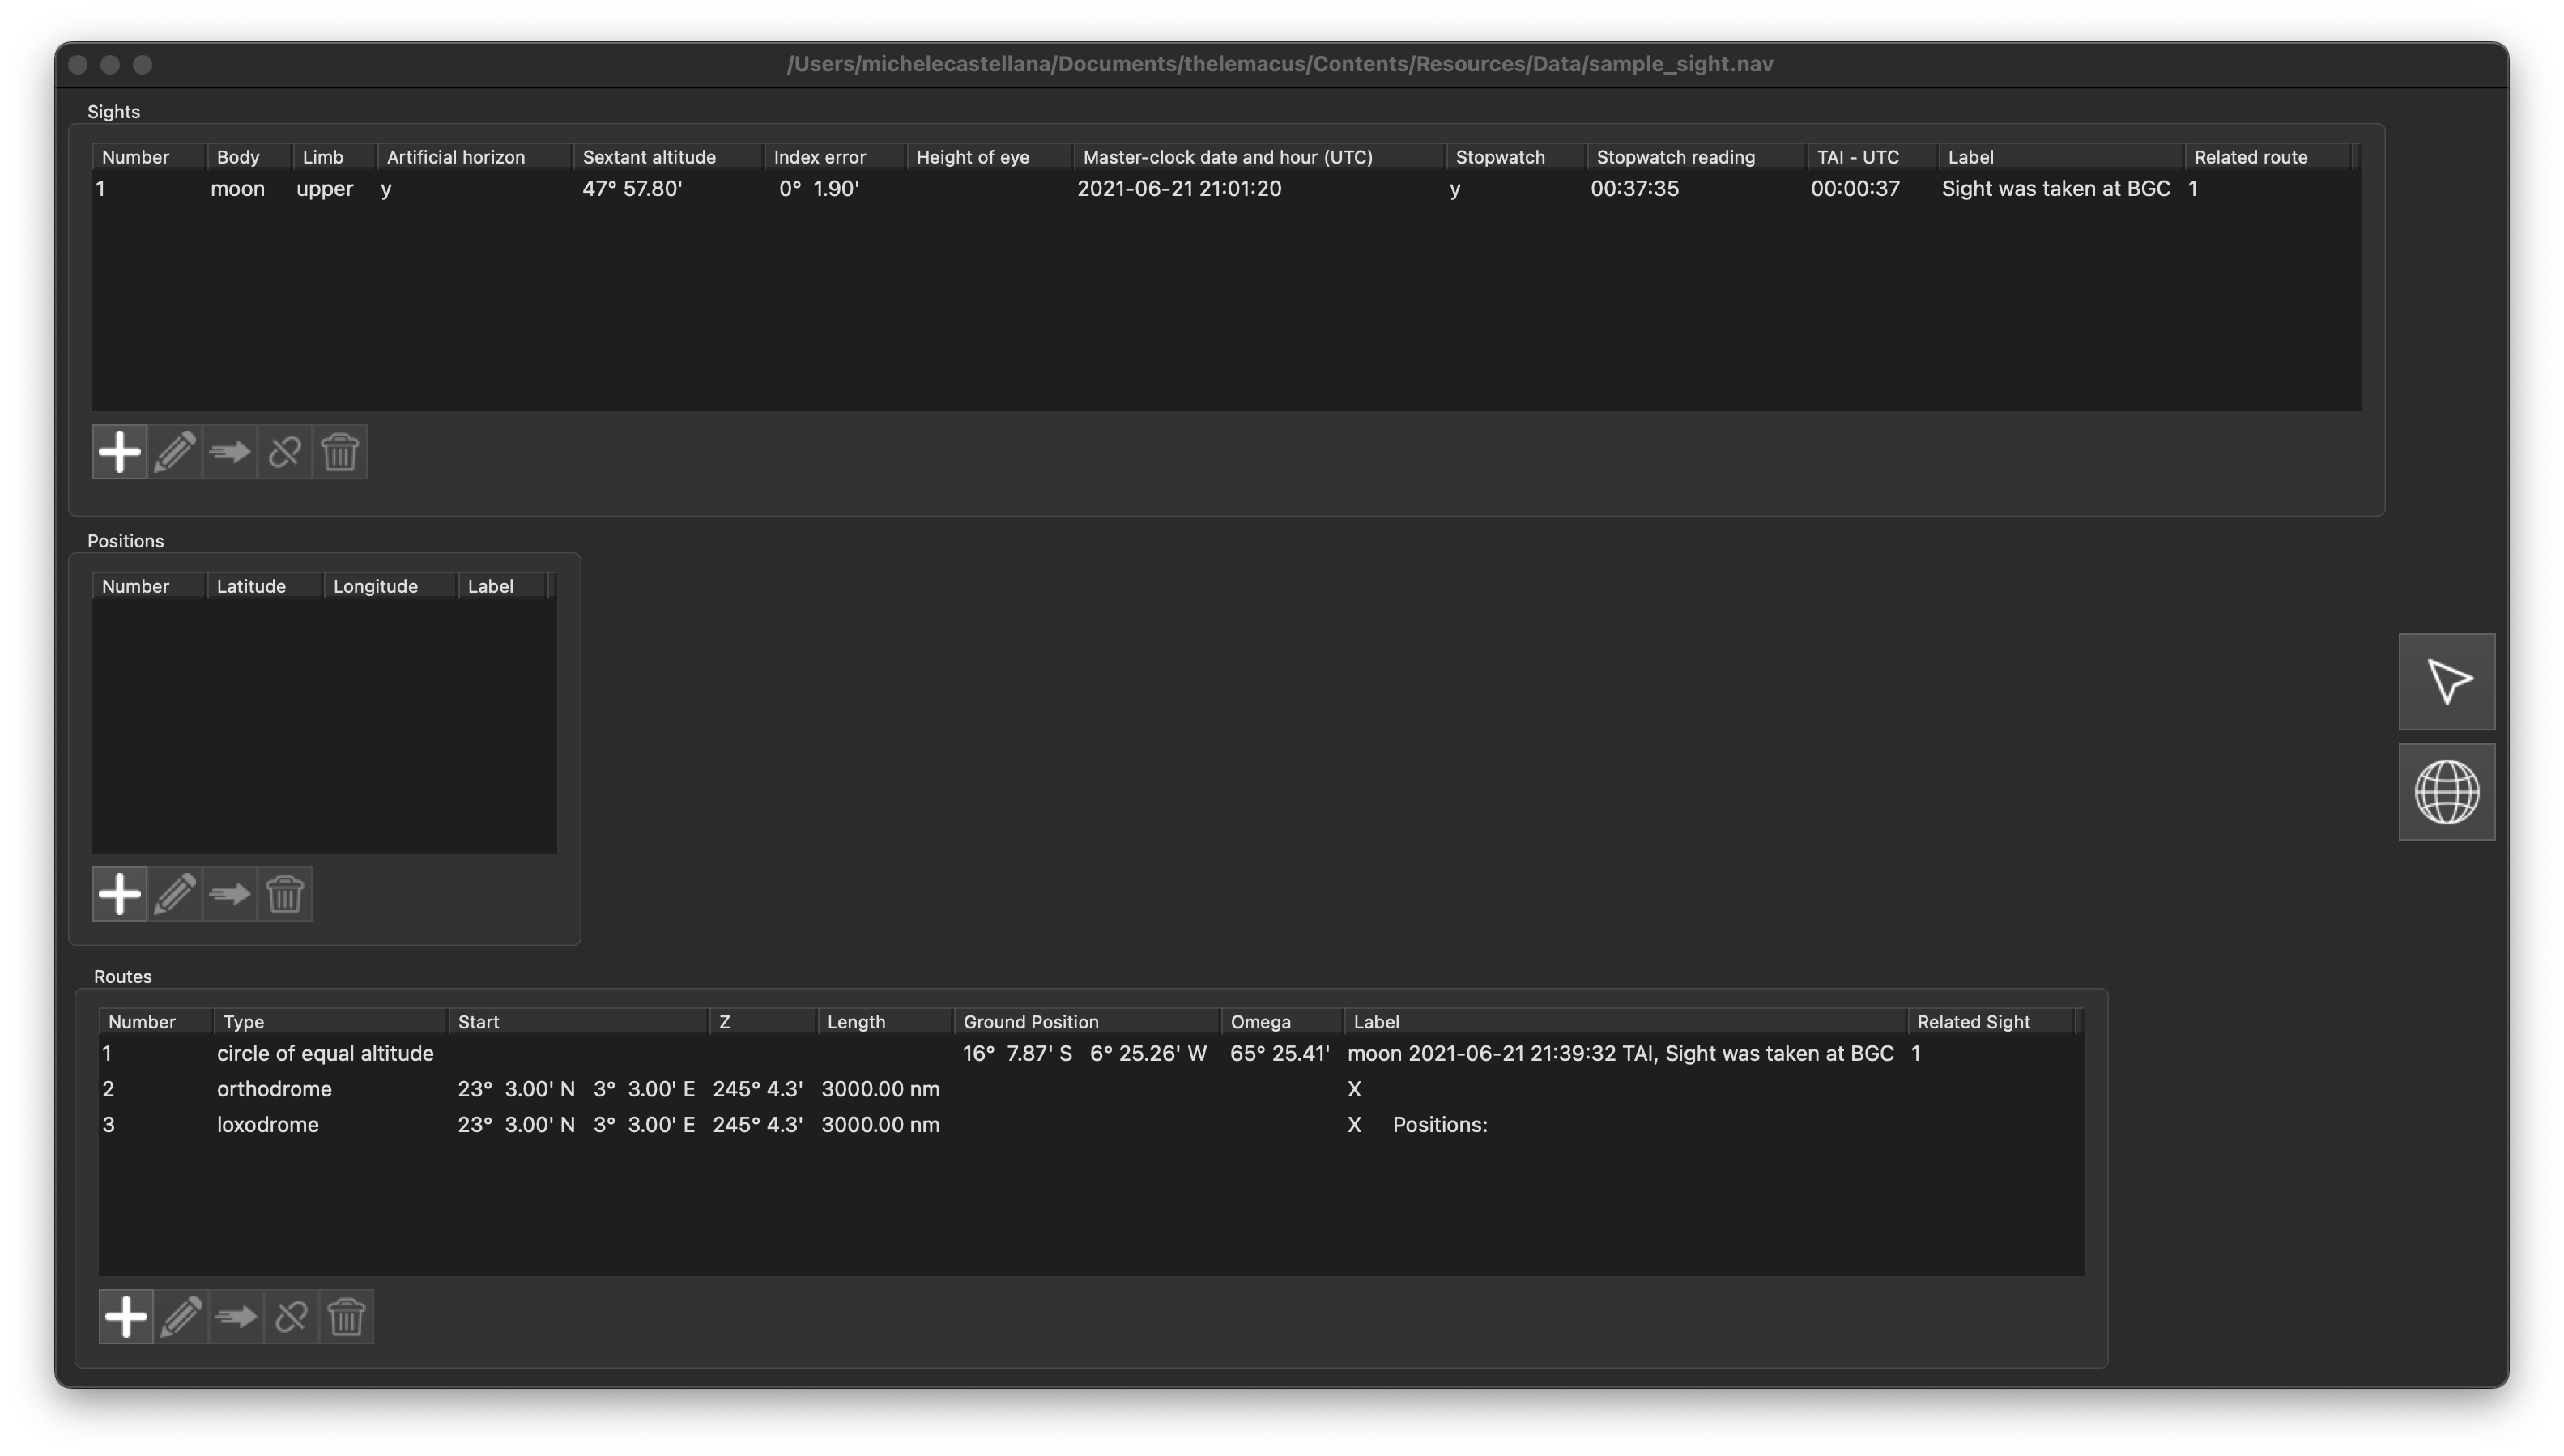
\includegraphics[width=1\textwidth]{figures/list-frame.png}
  \caption{
    \label{fig-list-frame}
    The main frame of \thel. 
  }
  \end{figure}


  \begin{figure}
    \centering
    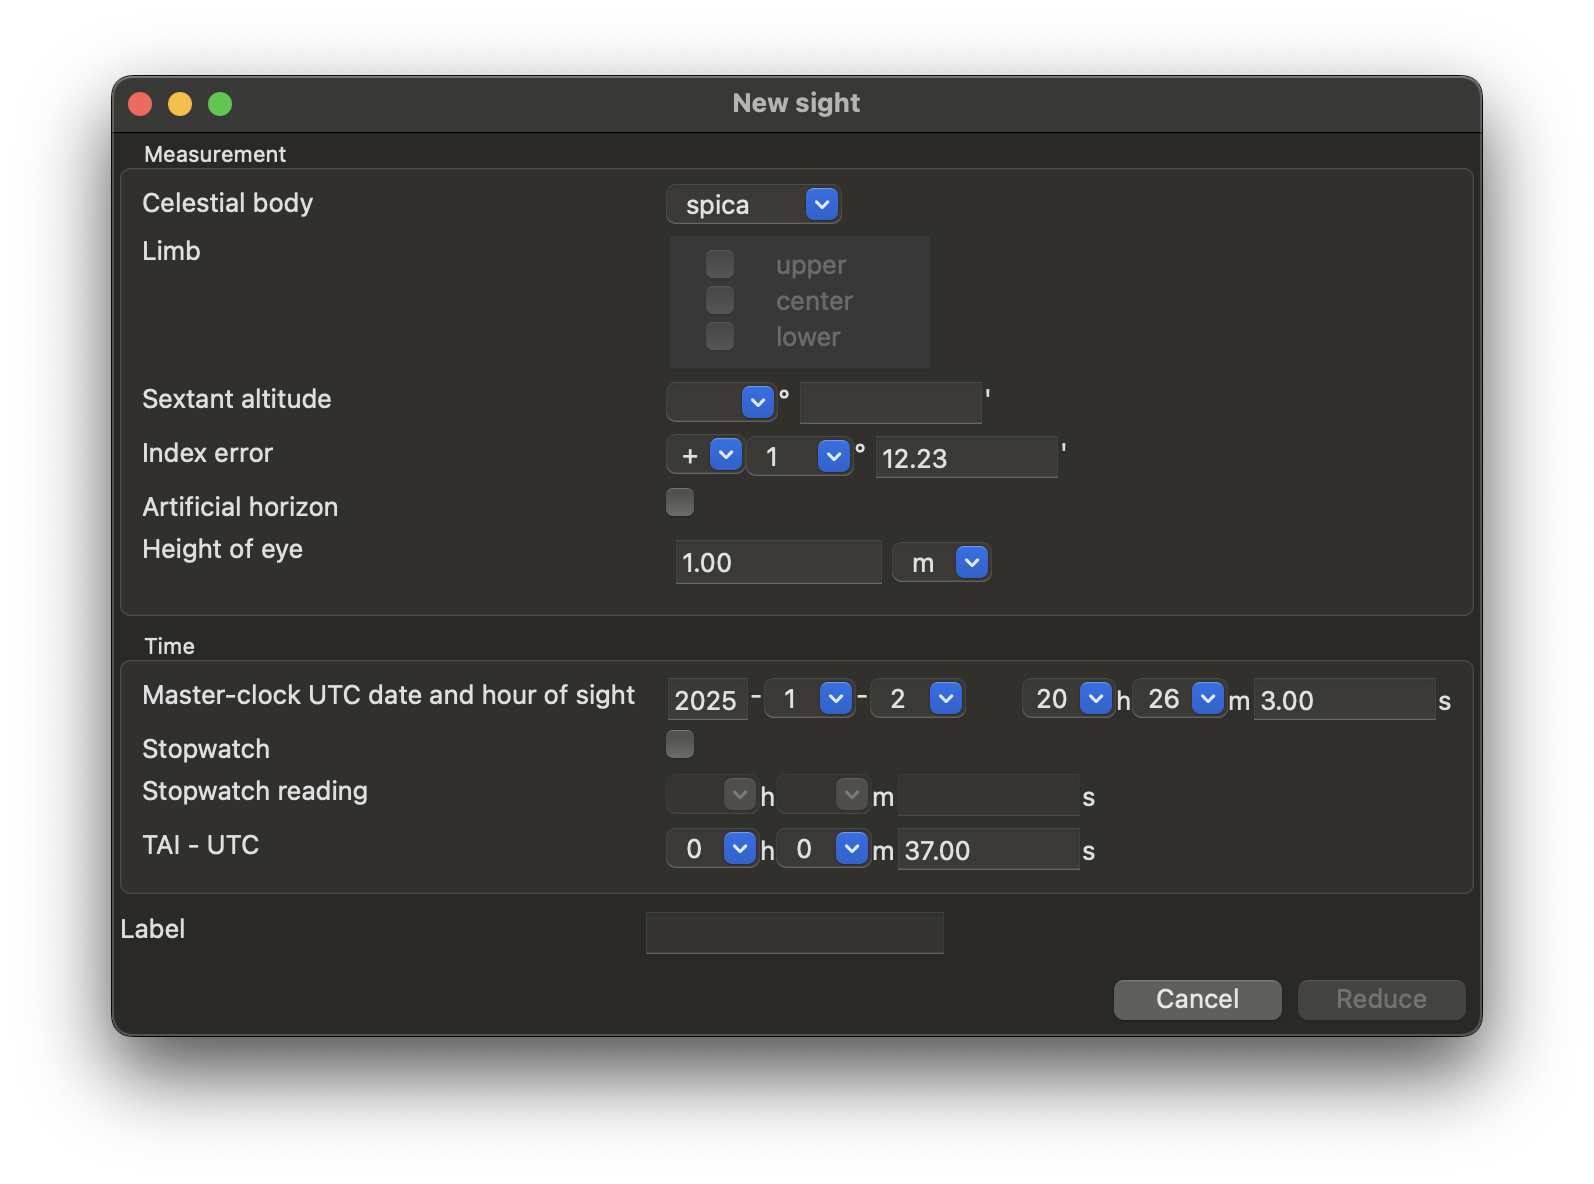
\includegraphics[width=0.9\textwidth]{figures/sight-frame.png}
    \caption{
      \label{fig-sight-frame}
      The sight frame with the entered data from \cref{item-name,item-limb,item-body-height,item-artificial-horizon,item-time,item-label,item-index-error,item-observer-height,item-tai-utc,item-stopwatch,item-tai-utc}. 
    }
  \end{figure}
  

For a quick use of \thel, the user may enter a sextant sight, with which he/she must be familiar, by going on the main frame of \cref{fig-list-frame} an clicking on \inlinefigure{figures/plus-button.png}. A sight frame will appear, see \cref{fig-sight-frame}, where the user will enter
\begin{enumerate}
  \item \label{item-name} The name of the celestial body, e.g. the star `Arcturus'
  \item \label{item-limb}  If the body is the Sun or the Moon, the limb (`upper', `center' or `lower') of the body which has been considered in the measurement
  \item \label{item-body-height} The angular height of the  body over the horizon, expressed in degrees and arcminutes, e.g., $54 \degree \, 45.34'$
  \item \label{item-artificial-horizon} Whether the observer used an artificial horizon or not for the measurement
  \item \label{item-time} \ac{UTC} date and time of the measurement, e.g., $2024$-$11$-$4$ $22$:$04$:$23$ \ac{UTC}
  \item \label{item-label} A label (optional), e.g., `First sight of my night shift'
  \end{enumerate}
  
  Additional information, which is most likely the same across multiple sights, is: 
  \begin{enumerate}[resume]
    \item \label{item-index-error} The index error \cite{bowditch2002the} of the sextant,  i.e., and angle expressed in degrees and arcminutes, e.g., $0 \degree \, 1.34'$
    \item \label{item-observer-height} The height of the observer above sea level, e.g. $32.3$ \acp{ft}
    \item \label{item-stopwatch} Whether the observer has used a stopwatch or not and, if so, the reading of the stopwatch, e.g., $1\hr \, 34 \min \, 12.43 \sec$
    \item \label{item-tai-utc} The difference between \ac{TAI} and \ac{UTC} at the time of the measurement, e.g., $00$:$00$:$34$. 
  \end{enumerate}

  Then click on \inlinefigure{figures/reduce-button.png}: \thel will highglight for the user a curve on the surface of the Earth; the user is located somewhere on that curve. 

To compute one's position, repeat the procedure above with another sextant sight, click on \inlinefigure{figures/position-button.png} in the main frame, and select \inlinefigure{figures/all-routes.png}: \thel will show on the chart the position, and list its coordinates in the `Positions' box in the main frame. 


\section{Using \thel}


In order to use the full potential of \thel, we encourage the user to get familiar with the following simple concepts, see \cite{bowditch2002the} for details. 

\subsection{Sights, positions and routes}

Let us get familiar with three basic concepts: 
\subsubsection{Sights} \label{section-sights} 

A \textit{sight} is a measurement of the angular altitude of a celestial body, made with a sextant. 
The results of this measurements are given in  \cref{item-name,item-limb,item-body-height,item-artificial-horizon,item-time,item-label,item-index-error,item-observer-height,item-tai-utc,item-stopwatch,item-tai-utc}. 


\subsubsection{Positions}  \label{section-positions} 

A \textit{position} a  location on the surface of the Earth, specified by 
\begin{itemize}
\item latitude and longitude, e.g., $54 \degree \, 45.34'\, \textrm{N}$ $23 \degree \, 5.33'\, \textrm{E}$,
\item a label (optional).
\end{itemize}
\subsubsection{Routes} \label{section-routes} 

A \textit{route} a trajectory on the surface of the Eearth, specified by 
\begin{enumerate}
  \item \label{item-route-type} The route type \cite{bowditch2002the}, which can be 
  \begin{enumerate}
  \item a loxodrome: a trajectory forming a constant angle with the meridians,
  \item an orthodrome: a part of a great circle,
  \item  a circle of equal altitude: a curve on the surface of the Earth from which an observer would see a celestial body at a given altitude above the horizon,
  \end{enumerate}
  \item \label{item-route-azimuth} The azimuth $Z$, i.e., the angle between the route  and the local meridian at the route starting position, e.g., $254 \degree \, 5.44'$,
  \item \label{item-route-length} The length, e.g., the length of the route sailed, which can be specified in two ways:
  \begin{enumerate}
  \item by providing the time and speed of the ship, e.g.  $01$:$23$:$33$ and $5$ \acp{kt}, from which  \thel will extract the length sailed,  
  \item by providing directly the length sailed by the ship  $15$ \acp{nm}. 

  \end{enumerate}

  \item \label{item-route-reference-position} The start position (for loxodromes and orthodromes) or the ground position (for circles of equal altitude), see \cref{section-positions},
  \item \label{item-route-aperture} For circles of equal altitude the aperture angle `omega',
  \item \label{item-route-label} A label (optional). 
\end{enumerate}

\begin{figure}
  \centering
  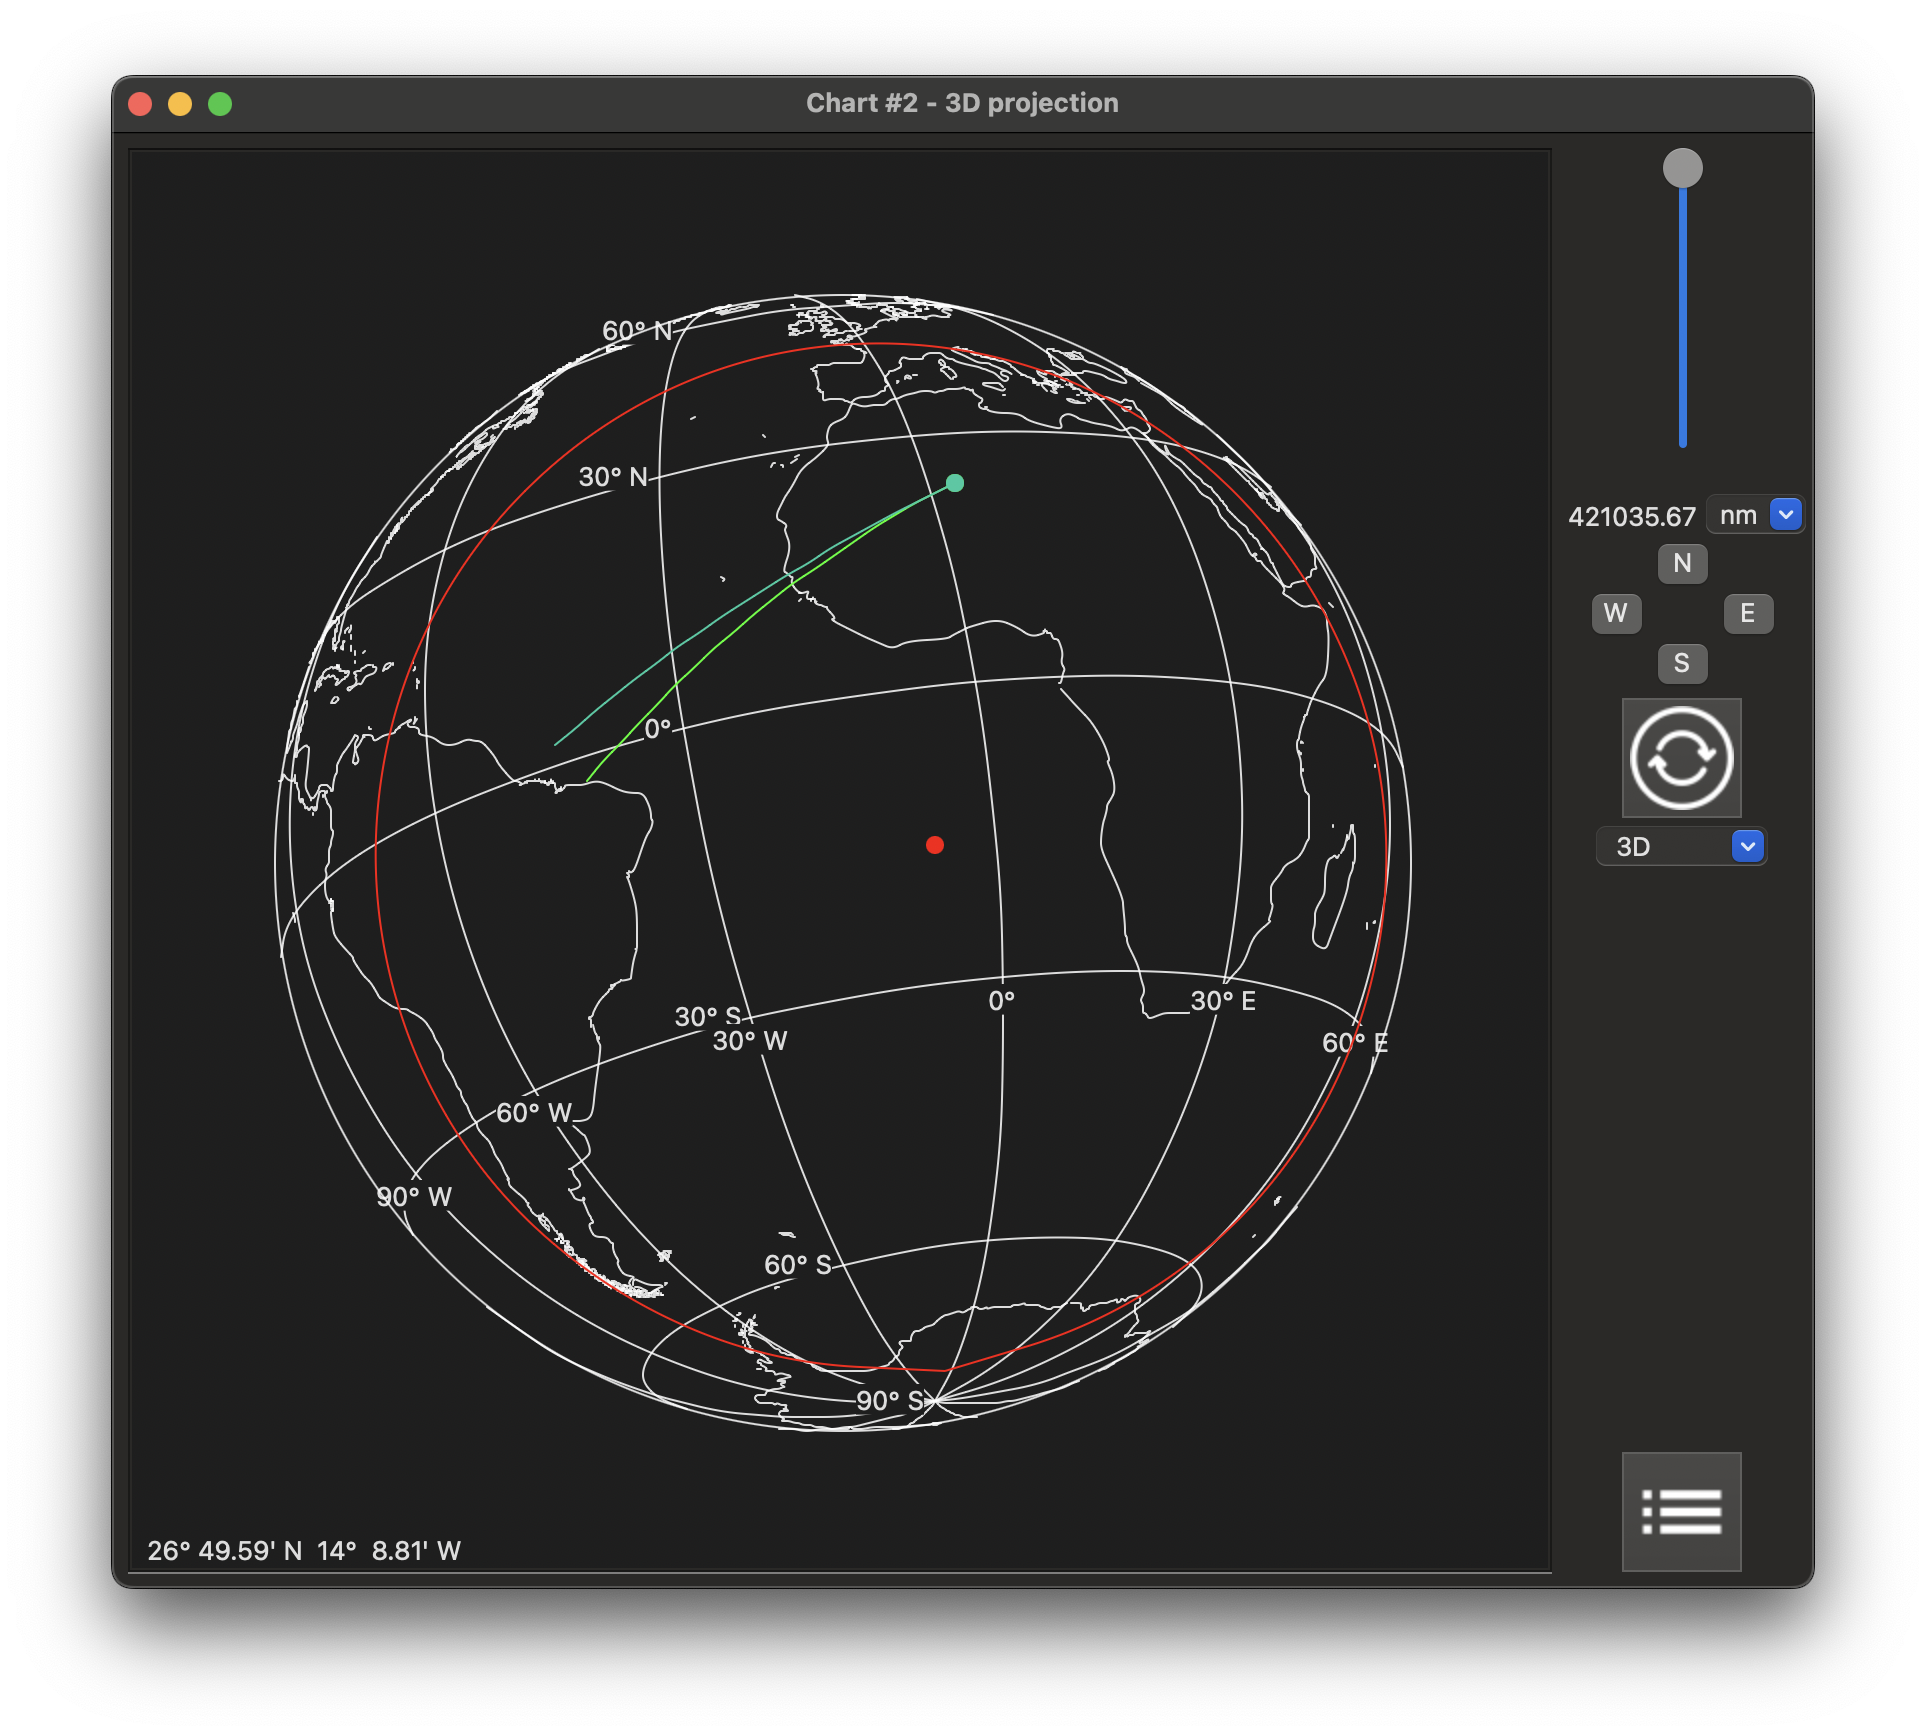
\includegraphics[width=0.9\textwidth]{figures/route-types.png}
  \caption{
    \label{fig-route-types}
    Three different route types: A loxodrome and an orthodrome with the same starting point (blue and green, respectively), and a circle of equal altitude (red), see \cref{item-route-type}. 
  }
  \end{figure}


When the observer takes a sight, then we can conclude that he/she lies on a route---a circle of equal altitude---on the Earth's surface \cite{bowditch2002the}. 
\textit{Reducing} a sight means computing this route given the sight data in \cref{item-route-reference-position}: we will say that this route is \textit{connected} to the sight. Importantly, not all routes are connected to sights: for example, a route denoting the ship's path, or a circle of equal altitude originally connected to a sight which has been later transported, are not. 

\subsection{The main frame}

\thel main frame is shown in \cref{fig-list-frame}. It is composed of three boxes: 
\begin{enumerate}
  \item \label{item-sight-box} Sight box: a table which contains the list of sights, i.e., sextant measurements. 
  
  Each line in the table corresponds to a sight, and its columns are given by: The sight identifier, which is automatically assigned by \thel,  the data in \cref{item-name,item-limb,item-body-height,item-artificial-horizon,item-time,item-label,item-index-error,item-observer-height,item-tai-utc,item-stopwatch,item-tai-utc}, and the identifier if the route related to the sight, see \cref{item-route-box}. 

  To enter a new sight, press the \inlinefigure{figures/plus-button.png} button at the bottom of the box. To modify or delete an existing sight, press  \inlinefigure{figures/modify-button.png} or  \inlinefigure{figures/delete-button.png}, respectively. To transport a sight, press \inlinefigure{figures/transport-button.png}. 
   To disconnect a sight from its route, press  \inlinefigure{figures/disconnect-button.png}. 

  \item \label{item-position-box} Position box: a table which contains the list of entered positions. 
  
  Each line corresponds to a position, and its columns are given by: The position identifier, automatically assigned by \thel,  latitude, longitude, and eventually a label. 

To add a new position, modify, transport or delete it, use the buttons at the bottom of the box. 

  \item \label{item-route-box} Route box: Each line corresponds to a route, and its columns are given by: The route identifier, automatically assigned by \thel, the data in \cref{item-route-type,item-route-azimuth,item-route-length,item-route-reference-position,item-route-aperture,item-route-label}. 
  \item 
  To add a new route, modify, transport, disconnect it from its sight or delete it, use the buttons at the bottom of the box. 

\end{enumerate}



If you hover the mouse over a sight in the sight box, the sight will be highlighted. The route to which it is connected, both in in the route box and in the chart frame, will be highlighted so the user can see directly to what route the sight corresponds on the chart. Positions and routes are highlighted in the same way. 


To compute the astronomical position, press \inlinefigure{figures/position-button.png}, and to jump to the charts, press \inlinefigure{figures/chart-button.png}.  

\subsection{Dealing with sights}

\subsubsection{Entering a sight: The sight frame}


To enter a new sight, press  \inlinefigure{figures/plus-button.png}, see \cref{fig-list-frame}, a sight frame will appear as in \cref{fig-sight-frame}, enter the sight fields in  \cref{item-name,item-limb,item-body-height,item-artificial-horizon,item-time,item-label,item-index-error,item-observer-height,item-tai-utc,item-stopwatch,item-tai-utc}, and press \inlinefigure{figures/reduce-button.png}. 

\textbf{\thel will produce, as output, a route}, and trigger a chart animation to it; \textbf{the observer is located  on this route}. This route is a circle of equal altitude, see \cref{fig-route-types}. 

\subsubsection{Astronomical fix}

By making multiple sights, one obtains multiple circles of equal altitude: the astronomical position is the crossing point between them---this procedure is called a \textit{fix}. 

To make an astronomical fix, click on \inlinefigure{figures/position-button.png} in the main frame: the position will be added to the position list with label `Astronomical position', and the charts will display it, see \cref{fig-astronomical-position}. The error on the astronomical position is a circle around it, and added to the route list. 

\begin{figure}
  \centering
  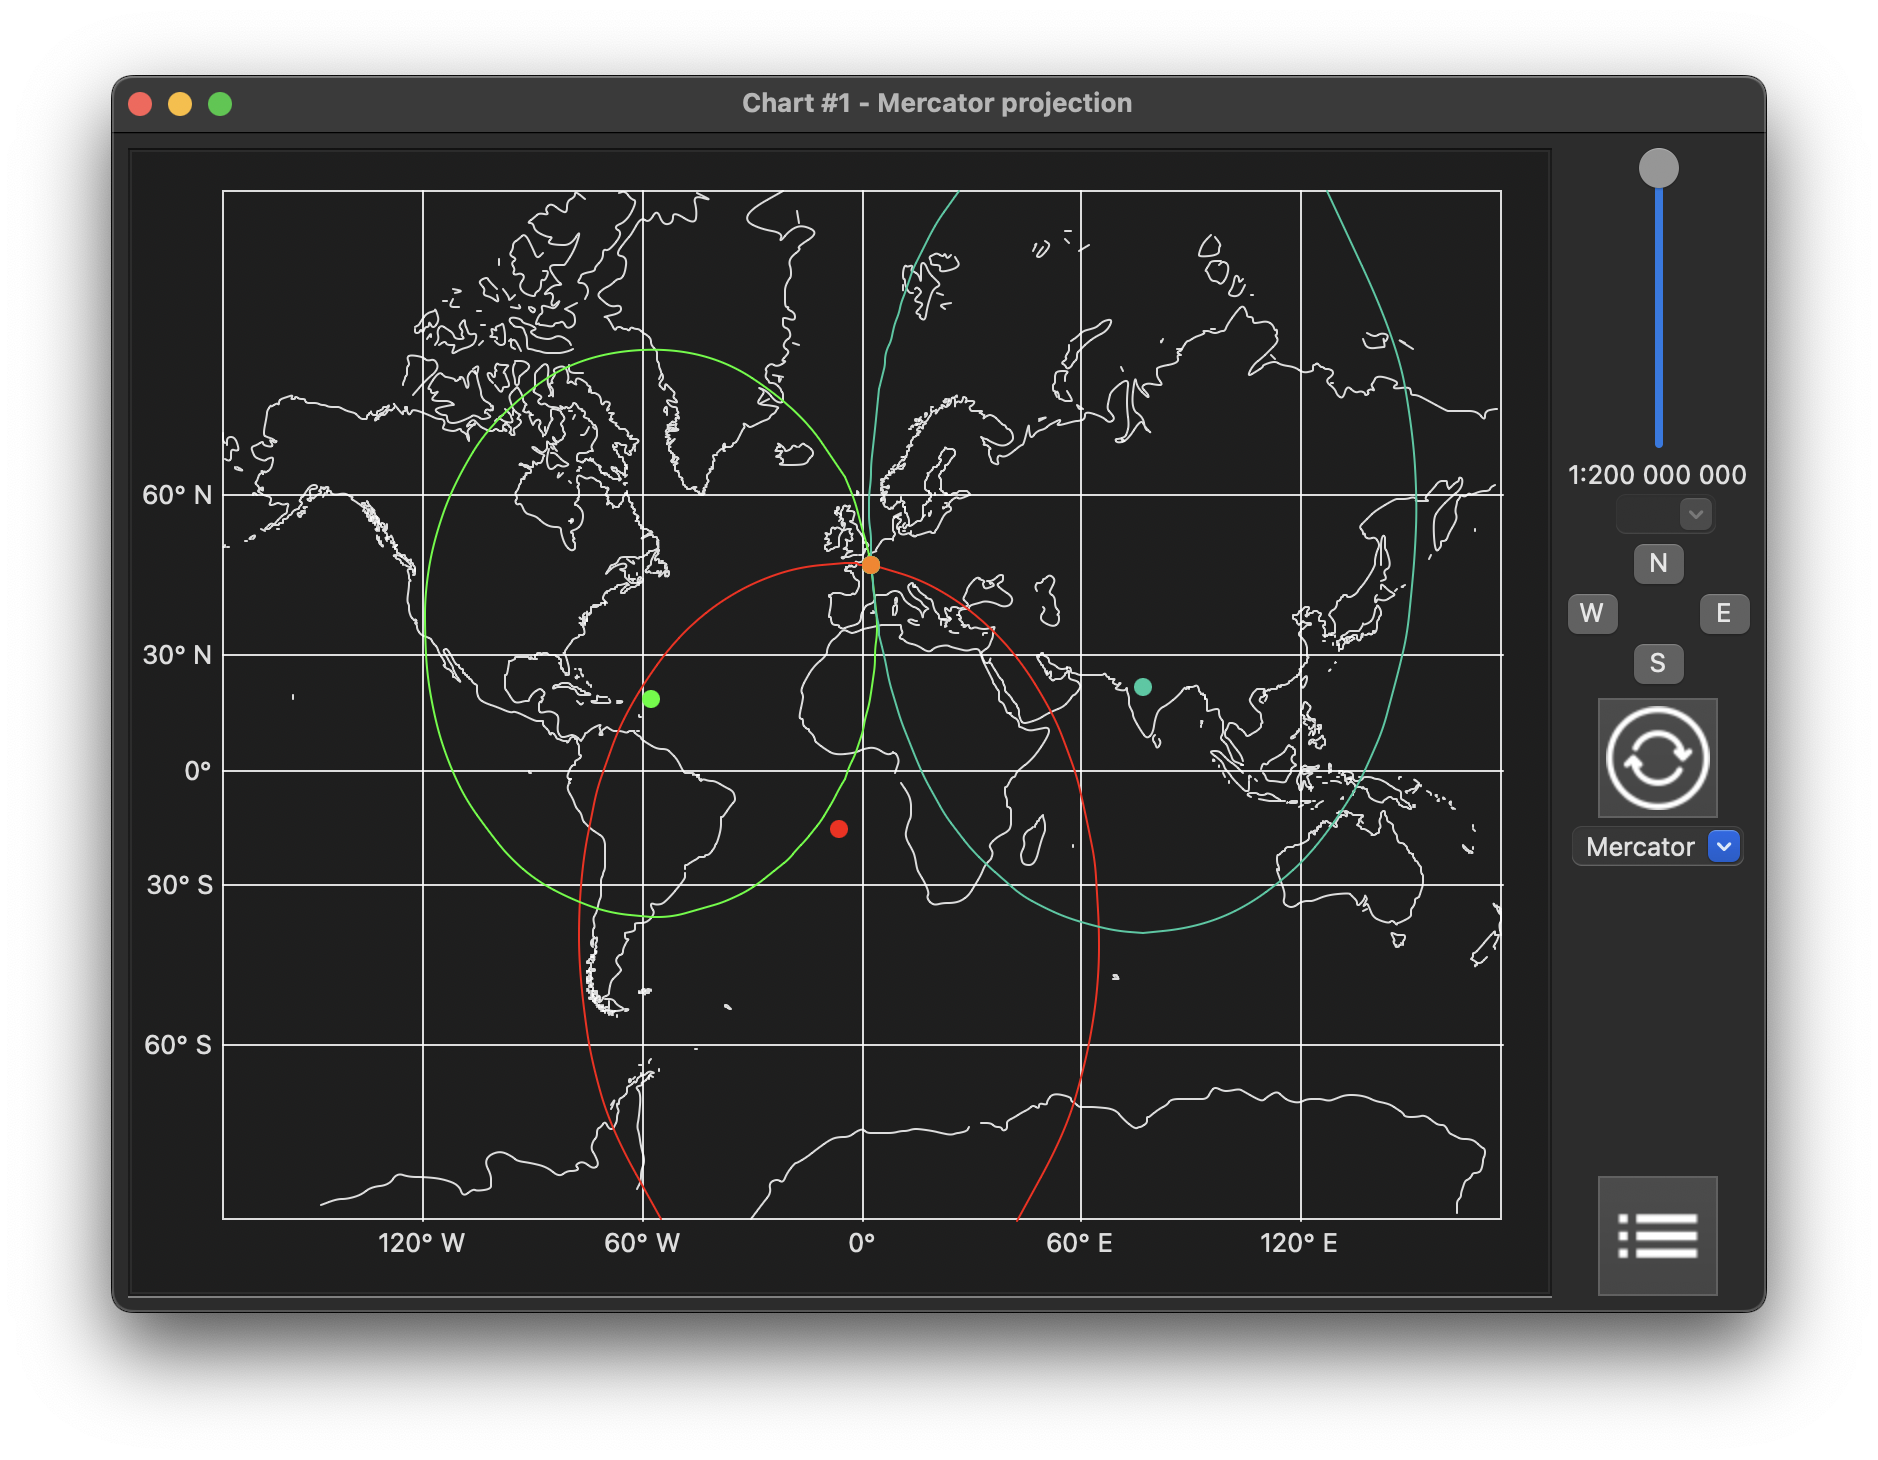
\includegraphics[width=0.9\textwidth]{figures/astronomical-position-mercator.png}
  \caption{
    \label{fig-astronomical-position}
    The crossing of the three routes (red, green and blue) yields the astronomical position (red dot located at the routes' crossing).  
  }
\end{figure}


\subsubsection{Transporting a sight}\label{section-transporting-sight}

If the course and speed of the ship are known, a sight taken in the past can be \textit{transported} and used after it was taken \cite{bowditch2002the,noauthor2017cours}. 

For example, suppose that the observer takes a Sun sight (A) in the afternoon, and then a Moon sight at dawn (B). Sight A can be transported along the route which the ship sailed between the time of A and that of B. The ship position at the time of B is the crossing between A transported and B. 

To transport a sight: 
\begin{itemize}
\item Click on the sight in the main frame
\item Click on \inlinefigure{figures/transport-button.png} at the bottom of the sight box. You can transport the sight
\begin{itemize}
\item with a route which is already in the route box, then press \inlinefigure{figures/existing-route-button.png}. Then confirm and select the route with which to do the transport by either
\begin{itemize}
  \item double clicking on it, or
  \item selecting it and pressing Enter on the keyboard. 
\end{itemize}
\item with a new route which you will create, then press 
\includegraphics{figures/new-route-button.png}, enter the information in the route frame, and press 
\includegraphics{figures/routeframe-transport-button.png}. 
\end{itemize}
\end{itemize}
An animation will move the transporting route in place, then transport the route sight, and move back the transporting route to its original position. 


\subsection{Dealing with positions}\label{section-position}

\begin{figure}
  \centering
  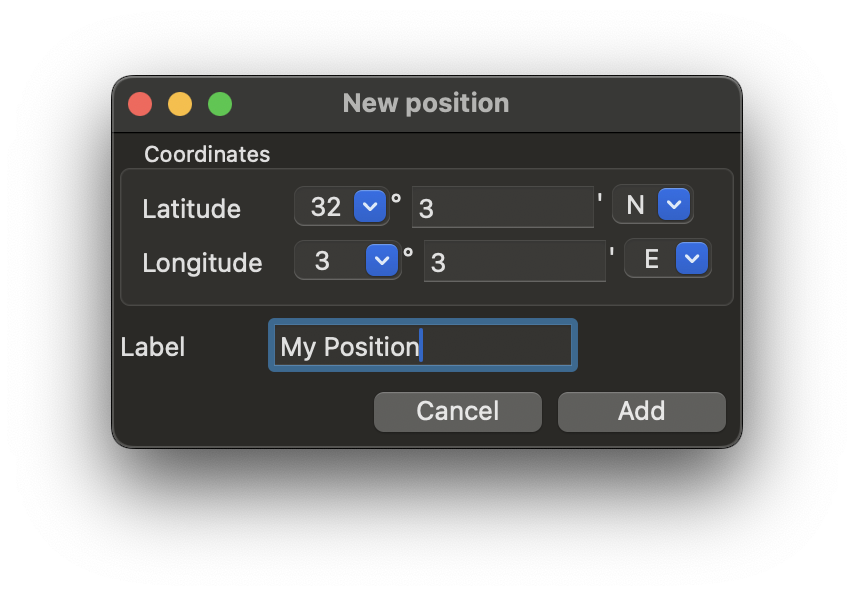
\includegraphics[width=0.5\textwidth]{figures/position-frame.png}
  \caption{
    \label{fig-position-frame}
    The position frame.  
  }
\end{figure}

\subsubsection{Entering a position}\label{section-enter-position}

To enter a position  (for example, the last estimated position, or the position where something worthwhile happened), go on the main frame and click on \inlinefigure{figures/plus-button.png} at the bottom of the position frame. The position frame will appear, see \cref{fig-position-frame}. Fill in the position fields of \cref{section-positions} and press \inlinefigure{figures/add-button.png}. 

\subsubsection{Transporting a position}\label{section-transport-position}

A position can be transported with a route along the lines of a sight transport, cf. \cref{section-transporting-sight}. This is useful, for instance, if one needs to transport the a past fix according to the recently sailed route, in order to obtain the current ship's position \cite{bowditch2002the}. 


\subsection{Dealing with routes}\label{section-routes}


\subsubsection{Entering a Route}\label{section-entering-route}

\begin{figure}
  \centering
  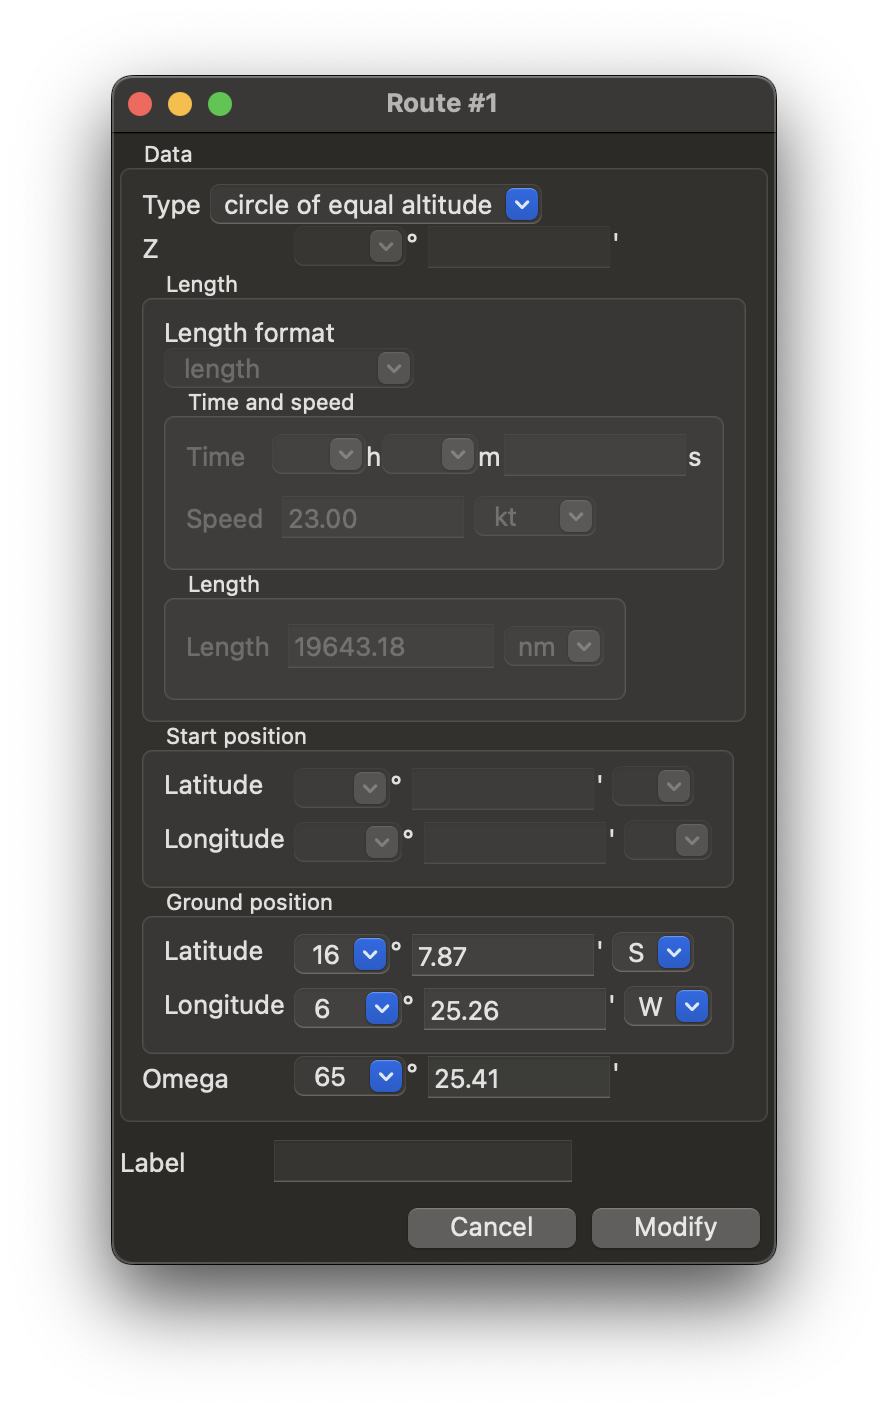
\includegraphics[width=0.5\textwidth]{figures/route-frame.png}
  \caption{
    \label{fig-route-frame}
    The route frame.  
  }
\end{figure}


To enter a route, go on the main frame and click on \inlinefigure{figures/plus-button.png} at the bottom of the route frame. The route frame will appear, see \cref{fig-route-frame}. Fill in the route fields of \cref{section-positions} and press \inlinefigure{figures/add-button.png}. 

\subsubsection{Transporting a Route}\label{section-transporting-route}

A route can be transported with another route along the lines of a sight and position transport, cf. \cref{section-transporting-sight,section-transport-position}. This is useful, for instance, if one needs to transport the a  circle of equal altitude of a past sight according to the recently sailed route, in order to obtain the current circle of equal altitude \cite{bowditch2002the}. 

%%%%%%%%

\pagebreak
\printacronyms[pages={display=all,seq/use=false}]
\bibliographystyle{unsrt}
%\addcontentsline{toc}{section}{\refname}
\bibliography{/Users/michelecastellana/Dropbox/my_bibliography/bibliography}


\end{document}
